\chapter{全志A83t Camera开发}
\begin{center}
纸上得来终觉浅,绝知此事要躬行。
\end{center}

\begin{flushright}
---傅玄
\end{flushright}

\section{总线与硬件接口}

根据全志官方提供的《A83t\_User\_Manual》和《A83t\-Datasheet》两个文档,可以知道A83t支持MIPI-CSI
总线和CSI总线,且A83t内部支持ISP,A83t体系架构图如图4.1所示。

\begin{figure}[!hbtp]
\centering
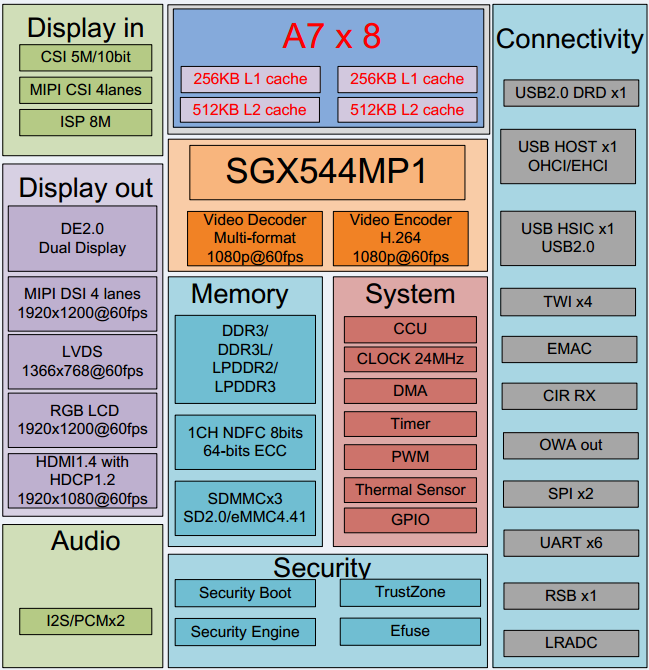
\includegraphics[width=0.8\textwidth]{Achitechture.png}
\caption{A83t体系架构\label{figur:A83t_Achitechture}}
\end{figure}

CSI接口的特性如图4.2,
\begin{figure}[H]
\centering
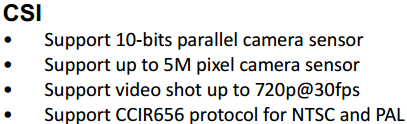
\includegraphics[width=0.8\textwidth]{CSI_feature.png}
\caption{CSI接口特性\label{figur:CSI_feature}}
\end{figure}

MIPI-CSI接口的特性如图4.3,
\begin{figure}[H]
\centering
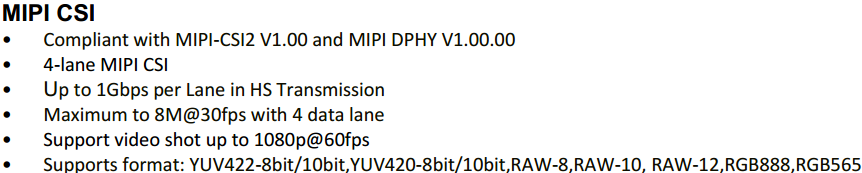
\includegraphics[width=0.8\textwidth]{MIPI-CSI_feature.png}
\caption{MIPI-CSI接口特性\label{figur:MIPI-CSI_feature}}
\end{figure}


\section{硬件原理图}
在调试的开发板上采用的是gc2145+gc0329连接到A83t的CSI0接口,gc2145器件原理图如图4.4所示,
\begin{figure}[H]
\centering
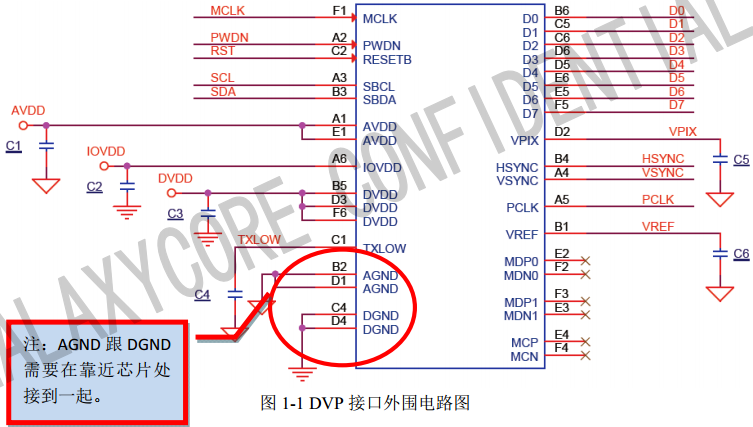
\includegraphics[width=0.8\textwidth]{GC2145.png}
\caption{GC2145器件原理图\label{figur:GC2145}}
\end{figure}
\section{驱动源码}

\section{内核与驱动配置}
调试camera需要配置内核与sysconfig.fex文件,内核配置如图4.6所示。
\begin{figure}[H]
\centering
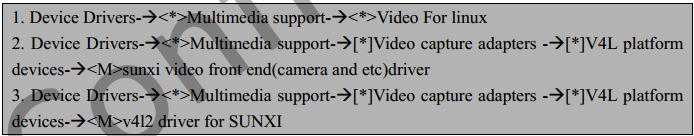
\includegraphics[width=0.8\textwidth]{menuconfig.png}
\caption{make menuconfig配置\label{figur:menuconfig}}
\end{figure}

除了基本的内核对camera的支持,还需要修改内核Makefile添加爱gc2145驱动的编译,修改文件路径:
linux-3.4/drivers/media/video/sunxi-vfe/device/Makefile,修改内容如图4.7所示,在24行添加了gc2145sensor模组的驱动编译,
\begin{figure}[H]
\centering
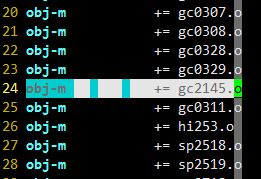
\includegraphics[width=0.8\textwidth]{gc2145_driver.png}
\caption{添加GC2145驱动\label{figur:gc2145_driver}}
\end{figure}

完成内核配置之后还需要对android系统进行配置,让android系统在启动时加载对应的驱动模块,对应的修改目录:
android/device/softwinner/octopus-f1/init.sun8i.rc,修改内容如图4.8所示,添加了加载gc2145.ko模块,去掉了ov5640模块的加载。
\begin{figure}[H]
\centering
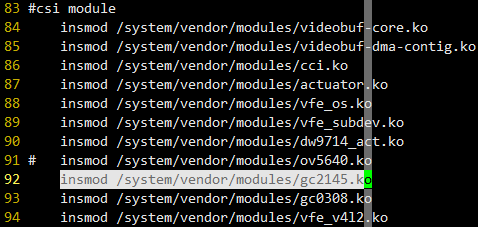
\includegraphics[width=0.8\textwidth]{android_init.png}
\caption{加载GC2145驱动\label{figur:android_init}}
\end{figure}

\section{调试问题记录}
将调试中遇到的一些问题记录如下:

\begin{enumerate}[1)]
\item \textbf{将sysconfig.fex文件配置好之后,编译固件下载运行,在linux加载时出现卡住无法启动的问题。}
\begin{figure}[H]
\centering
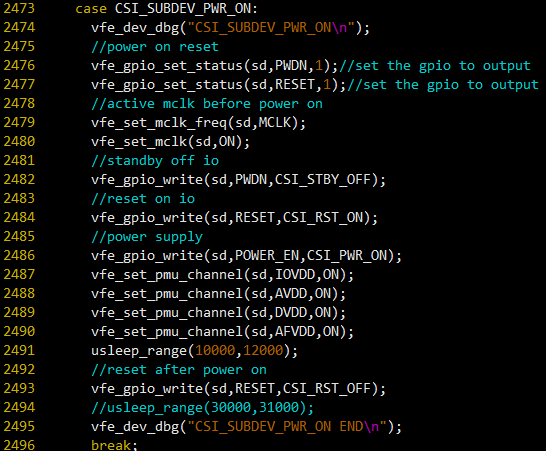
\includegraphics[width=0.8\textwidth]{bug_code01.png}
\caption{定位代码\label{figur:bug_code01}}
\end{figure}

解决方法:在各个驱动里面添加打印,定位具体是什么位置导致了CPU死掉,初步判断是有空指针之类的问题,但是内核栈没有更多的信息打印出来。
还想到一个办法,便是通过将android中设置的自动加载camera各个驱动,换成手动加载驱动,看看是如何挂掉的。
添加打印后和换成手动加载驱动之后定位到挂掉的代码位置,代码路径linux-3.4/drivers/media/video/sunxi-vfe/device/gc2145.c,
如图4.8所示,最后定位到了vfe\_set\_pmu\_channel(sd, IOVDD, ON)这一句,原来是在sys\_config.fex中iovdd-csi位置设置错误,放到了
aldo2下面,aldo2是控制sdram和pll的电源。

完成电源配置之后,摄像头便可以正常启动了,此时的sys\_config.fex的电源分配如图4.9所示,将iovdd-csi分配到了axp81x\_dldo3,将
dvdd-csi-18分配在了axp81x\_eldo1,avdd-csi分配在了axp81x\_dldo4。
\begin{figure}[htbp]
\centering
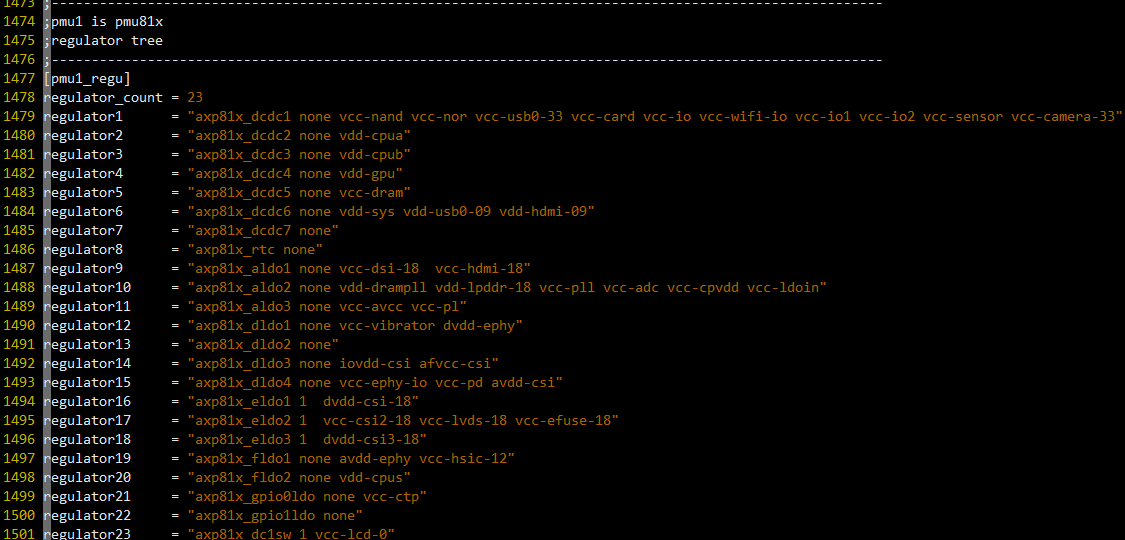
\includegraphics[width=0.8\textwidth]{sys_config0.png}
\caption{sys\_config电源分配\label{figur:sys_config0}}
\end{figure}

iovdd是摄像头模块io接口电源,avdd是摄像头模块模拟电路电源,dvdd是摄像头模块数字电路电源,具体电源配置电压如图4.10所示,
\begin{figure}[htbp]
\centering
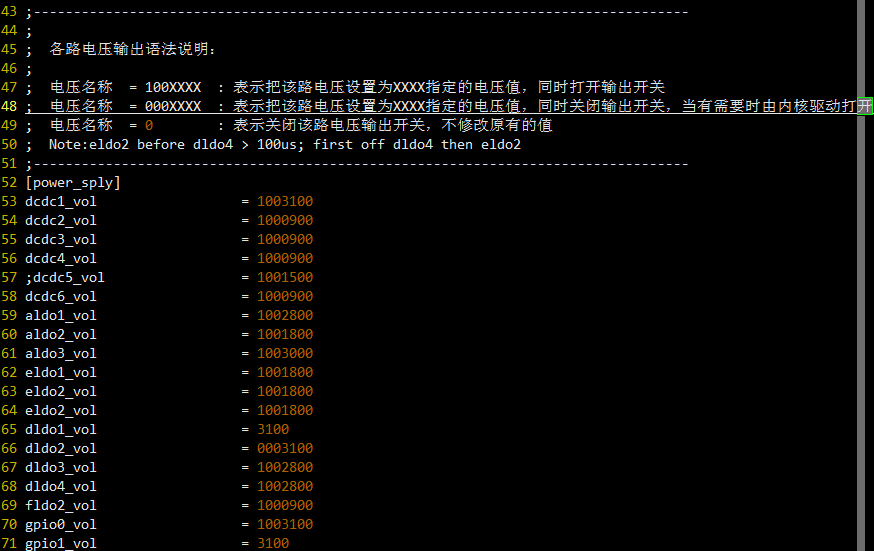
\includegraphics[width=0.8\textwidth]{sys_config1.png}
\caption{sys\_config电源电压配置\label{figur:sys_config1}}
\end{figure}



\item \textbf{驱动挂死}

解决方法:

\end{enumerate}

    
\section{总结}